\providecommand{\main}{..}
\documentclass[\main/notes.tex]{subfiles}

\begin{document}
	\setcounter{chapter}{6}
	\chapter{Operating Systems}
		\section{Introduction}
			Computers are made up of two major components: \concept{hardware} and \concept{software}.
			\begin{indentparagraph}
				\begin{description}
					\item[Hardware] The physical equipment.
					\item[Software] The collection of programs that allows hardware to do its job. Divided into the \concept{operating system}, and \concept{application programs}.
					\begin{indentparagraph}
						\begin{description}
							\item[Application Programs] Use the computer hardware to solve users' problems
							\item[Operating System] Controls access to hardware by users.
						\end{description}
					\end{indentparagraph}
				\end{description}
			\end{indentparagraph}
			\begin{definition}{Operating System}
				An interface between the hardware of a computer and the user (programs or humans), that facilitates the execution of other programs and the access to hardware and software resources.
			\end{definition}
			Two major design goals of an operating system are:
			\begin{indentparagraph}
				\begin{itemize}
					\item Efficient use of hardware
					\item Easy use of resources
				\end{itemize}
			\end{indentparagraph}
			\subsection{Bootstrap Process}
				The OS is a program itself, that needs to be loaded into memory.\par
				To do this, the manufacturer stores the OS in part of memory using ROM technology. The program counter of the CPU is set to the beginning of this ROM memory. This is inefficient, because a significant part of memory would need to be composed of ROM, and therefore could not be used by other programs.\par
				To solve this, a two-stage process is used. A very small section of memory is made of ROM, and holds a small program called the \concept{bootstrap program}. When the computer is turned on, the CPU counter is set to the first instruction of this bootstrap program. This program is only used to load the operating system itself -- the parts required to start up the computer -- into RAM memory. After is is loaded, the program counter is set to the first instruction of the operating system.

		\pagebreak
		\section{Evolution}
			\subsection{Batch Systems}
				\concept{Batch Operating Systems} were designed in the $1950$s to control mainframe computers.

				Each program to be executed is called a \concept{job}. To execute a job, a programmer sends a request to the operating room along with punched cards for the program and data. If the program is successful, a printout is sent to the programmer, otherwise a printout of the error is sent.
			\subsection{Time-Sharing Systems}
				To use computer resources more efficiently, \concept{multiprogramming} was introduced.
				\begin{indentparagraph}
					\begin{description}
						\item[Multiprogramming] Hold several jobs in memory at a time, and only assign a resource to a job that needs it on the condition that the resource is available.
						\item[Time Sharing] Resources can be shared between different jobs, with each job being allocated a portion of time to use the resource. Due to computer speed, this is hidden from a user -- each user has the impression that the whole system is serving them exclusively. 
					\end{description}
				\end{indentparagraph}
				Both of the above impove the efficiency of computer systems, but increased the complexity. The operating system now had to do \concept{scheduling}.
				\begin{indentparagraph}
					\begin{description}
						\item[Scheduling] Allocating resources to different programs, and deciding which program could use which resource, and when.
					\end{description}
				\end{indentparagraph}
				The relationship between a user and computer changes: the user can directly interact with the system without going through an operator.

				The concept of a \concept{process} is developed: a program that is in memory that is waiting for resources.
			\subsection{Personal Systems}
				When personal computers are introduced, \concept{single-user operating systems} are developed. An example is \concept{DOS (Disk Operating System)}.
			\subsection{Parallel Systems}
				The need for more speed and efficiency leads to the design of \concept{parallel systems}: multiple CPUs on the same machine. Each CPU can be used to serve one program or a part of a program -- many tasks can be accomplished in parallel rather than serially. The complexity of these operating systems increases.
			\subsection{Distributed Systems}
				Operating systems that use networking and internetworking. A job can be shared between different computers -- a program can run partially on one computer and partially on another. Resources can be distributed. \concept{Distributed systems} use features from the previous generations, along with new duties such as controlling security.
			\subsection{Real-time Systems}
				Expected to do a task within specific time constraints. Used with real-time applications, which monitor, respond to, or control external processes or environments.

		\section{Components}
			A modern operating system has at least four duties:
			\begin{indentparagraph}
				\begin{itemize}
					\item memory manager
					\item process manager
					\item device manager
					\item file manager
				\end{itemize}
			\end{indentparagraph}
			There is also the \concept{user interface} (or \concept{shell}) that is not under any specific manager.
			\begin{indentparagraph}
				\begin{description}
					\item[User Interface (Shell)] Responsible for communication outside the operating system.
				\end{description}
			\end{indentparagraph}
			\begin{center}
				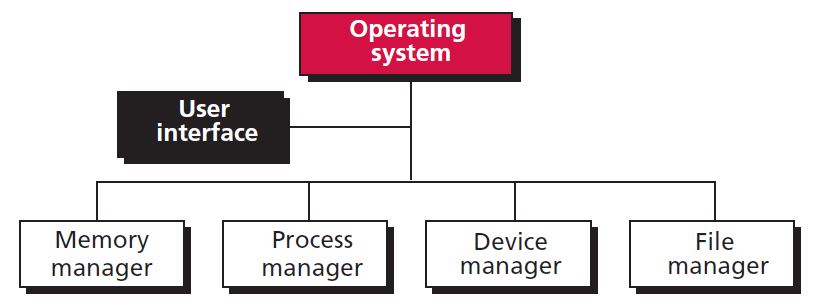
\includegraphics[width=0.9\textwidth]{\main/images/unit07/operating_system.png}
			\end{center}
			\subsection{User Interface}
				\begin{definition}{User Interface}
					A program that accepts requests from users (processes) and interprets them for the rest of the operating system.

					In some operating systems, such as UNIX, this is called a \concept{shell}. In others, it is called a \concept{window}, to denote that it is menu driven, and has a \concept{GUI (graphical user interface)}.
				\end{definition}
			\pagebreak
			\subsection{Memory Manager}
				To prevent applications from running out of memory, memory allocation must be managed. There are two broad categories for memory management: \concept{monoprogramming} and \concept{multiprogramming}.
				\subsubsection{Monoprogramming}
					Older method, not used now. Most of the memory is dedicated to a single program: only a small part is needed to hold the operating system.

					The entire program is in memory for execution. When the program finishes running, the program area is occupied by another program.
					\begin{center}
						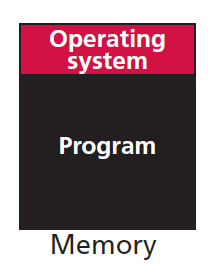
\includegraphics[width=0.2\textwidth]{\main/images/unit07/monoprogramming.png}
					\end{center}

					Memory manager loads the program into memory, runs it, and replaces it with the next program.

					Problems with this technique:
					\begin{indentparagraph}
						\begin{itemize}
							\item The program must fit in memory -- the size of the program cannot be bigger than the size of memory.
							\item When a program is being run, no other program can be executed. This is inefficient for the CPU and memory, especially if the CPU needs to wait for an I/O device.
						\end{itemize}
					\end{indentparagraph}
				\subsubsection{Multiprogramming}
					More than one program is in memory at the same time, and they are executed concurrently, with the CPU switching rapidly between the programs.
					\begin{center}
						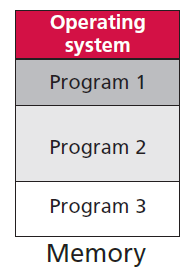
\includegraphics[width=0.2\textwidth]{\main/images/unit07/multiprogramming.png}
					\end{center}

					\pagebreak
					There are multiple different schemes for the way that multiprogramming can work: they can be classified as either \concept{nonswapping} or \concept{swapping}.
					\begin{indentparagraph}
						\begin{description}
							\item[Nonswapping:] Partitioning, and Paging
							\item[Swapping] Demand Paging, and Demand Segmentation
						\end{description}
					\end{indentparagraph}
					\begin{center}
						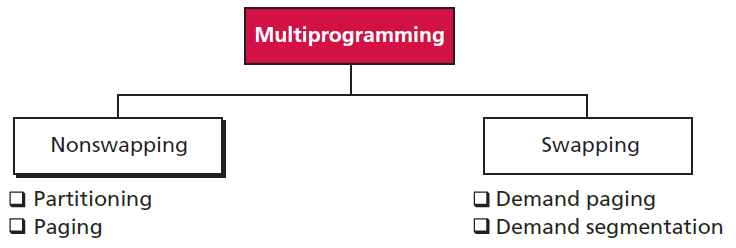
\includegraphics[width=0.7\textwidth]{\main/images/unit07/multiprogramming_categories.png}
					\end{center}
					\begin{definition}{Partitioning}
						Memory is divided into variable length sections, where each section (or \concept{partition}) holds one program.

						The CPU switches between programs. Start with one program, and continue execution until an I/O operation occurs, or the time allocated expires. Then it switches to the next program. Once all programs have been served, it moves back to the first program.

						Issues related:
						\begin{itemize}
							\item The size of the partitions is determined beforehand. If the partitions are too small, some programs can't be loaded into memory. If the partitions are too big, there are unused locations is memory.
							\item Even if perfect at the start, may be holes after a completed program is replaced in memory.
							\item If there are many holes, the memory manager can compact the partitions to remove the holes, but this creates extra overload on the system.
						\end{itemize}
					\end{definition}
					\pagebreak
					\begin{definition}{Paging}
						Improves the efficiency of partitioning. Memory is divided into equally sized sections called \concept{frames}. Programs are also divided into equally sized sections called \concept{pages}. The size of a page and a frame is usually the same, and equal to the size of the block used by the system to retrieve information from a storage device.

						A page is loaded into a frame in memory. If a program has three pages, it occupies three frames in memory.

						The program \emph{does not} have to be contiguous: two consecutive pages can occupy noncontiguous frames in memory.
						\begin{center}
							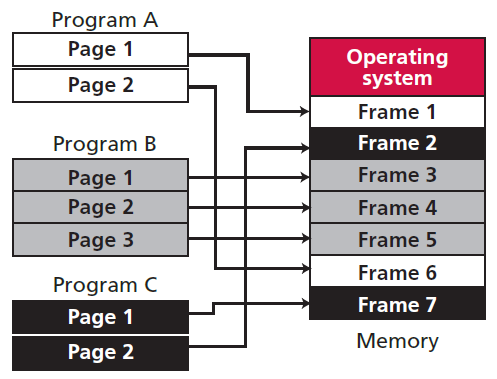
\includegraphics[width=0.5\textwidth]{\main/images/unit07/paging.png}
						\end{center}

						Paging improves efficiency, but the entire program still needs to be in memory before being executed.
					\end{definition}
					\begin{definition}{Demand Paging}
						Removes the restriction that the entire program needs to be in memory. The program is divided into pages, but the pages can be loaded into memory one by one, executed, and replaced by another page.
						\begin{center}
							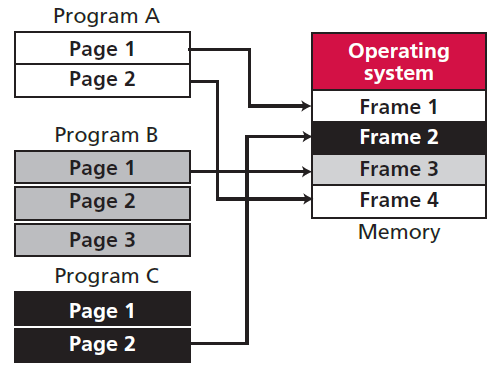
\includegraphics[width=0.5\textwidth]{\main/images/unit07/demand_paging.png}
						\end{center}
					\end{definition}
					\pagebreak
					\begin{definition}{Demand Segmentation}
						Instead of dividing a program into pages, a program is divided into \concept{segments} that reprent the modules of the program. These are loaded into memory, executed, and then replaced by another module from the same or a different program.

						Segments in memory are of the same size, which means that part of a segment may remain empty.
						\begin{center}
							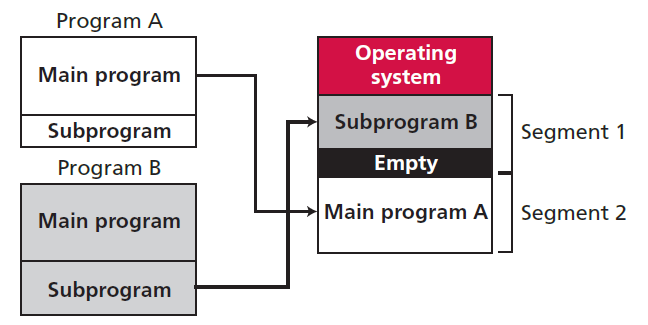
\includegraphics[width=0.7\textwidth]{\main/images/unit07/demand_segmentation.png}
						\end{center}
					\end{definition}
					\begin{sidenote}{Demand Segmentation and Demand Paging}
						These two techniques can be combined to improve the efficiency of the system. A segment may be too large, in which case memory can be divided into frames, and a module into pages. The pages of a module can then be loaded into memory one-by-one and executed.
					\end{sidenote}
					\begin{definition}{Virtual Memory}
						With \concept{demand paging} and \concept{demand segmentation}, part of the program is in memory, and part is on disk. While a smaller amount of a program is in actual memory at a specific time, a larger part on disk contains the parts not currently running. This larger part is called \concept{virtual memory}.
					\end{definition}
			\pagebreak
			\subsection{Process Manager}
				\begin{definition}{Program}
					A nonactive set of instructions stored on disk, or tape. It may or may not become a \concept{job}.
				\end{definition}
				\begin{definition}{Job}
					A program becomes a job from the moment it is selected for execution until it has finished running, and becomes a program again.

					During this time, a job may or may not be executed -- it may be on disk waiting to be loaded to memory, or in memory waiting for execution from the CPU.

					Every job is a program, but not every program is a job.
				\end{definition}
				\begin{definition}{Process}
					A program in execution. A program that has started, but not finished. A job that is being run in memory. It may be executing, or waiting for CPU time. As long as the job is in memory, it is a process.

					Every process is a job, but not every job is a process.
				\end{definition}
				\begin{center}
					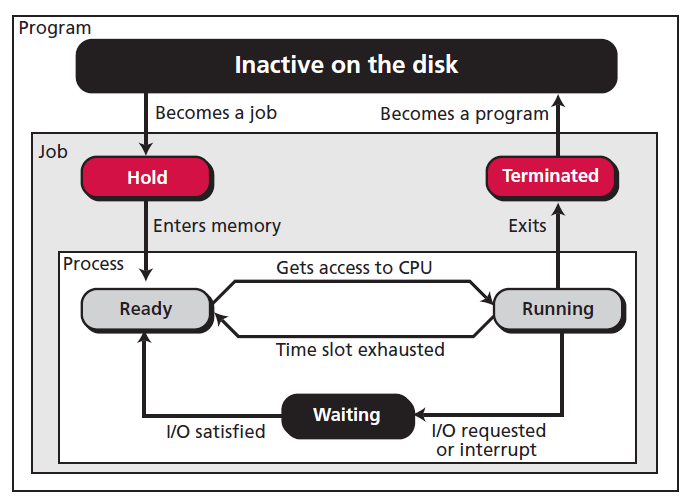
\includegraphics[width=0.6\textwidth]{\main/images/unit07/process_state_diagram.png}
				\end{center}
				A program becomes a job when selected by the operating system, and brought to the \concept{hold state}. It remains in this state until it can be loaded into memory.

				When there is memory space available to load the program, the job moves to the \concept{ready state}. It now becomes a process.

				It remains in this state until the CPU can execute it, when it moves to the \concept{running state}. In this state, one of three things can happen:
				\begin{itemize}
					\item The process executes until it needs I/O resources -- goes to the \concept{waiting state}
					\item The process exhausts its allocated time slot -- goes to the \concept{ready state}
					\item The process terminates -- goes to the \concept{terminated state}, and is no longer a process.
				\end{itemize}

				\subsubsection{Schedulers}
					To move a job or process from one state to another, the process manager uses two schedulers: the \concept{job scheduler} and the \concept{process scheduler}.
					\begin{definition}{Job Scheduler}
						Moves a job from the hold state to the ready state, or from the running state to the terminated state. Responsible for creating a process from a job, and terminating a process.
						\begin{center}
							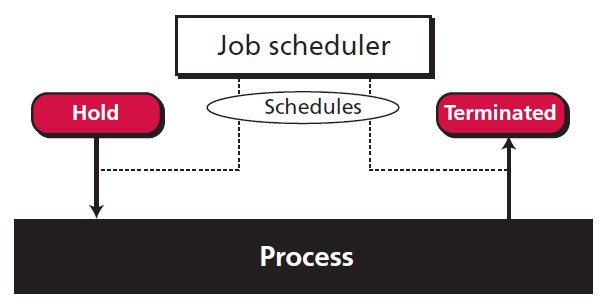
\includegraphics[width=0.5\textwidth]{\main/images/unit07/job_scheduler.png}
						\end{center}
					\end{definition}
					\begin{definition}{Process Scheduler}
						Moves a process from one state to another. Moves a process from the running state to the waiting state when the process is waiting for some event. Moves a process from the waiting state to the running state when the event has occured. Moves a process from the running state to the ready state if the time allotment has expired. Moves a process from the ready state to the running state.
						\begin{center}
							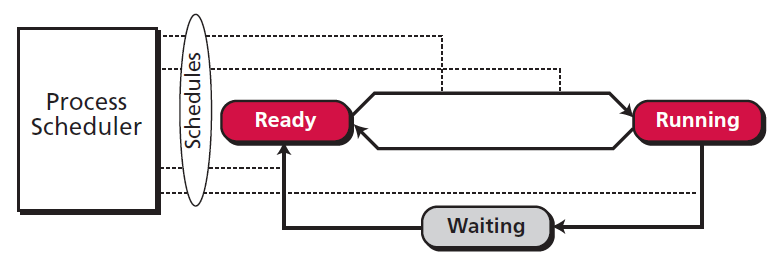
\includegraphics[width=0.6\textwidth]{\main/images/unit07/process_scheduler.png}
						\end{center}
					\end{definition}

				\subsubsection{Queueing}
					To handle multiple processes and jobs, the process manager uses \concept{queues}. A \concept{job control block}, or \concept{process control block} is associated with each job or process. This is a block of memory that stores information about that job or process. The process manager stores the control block in the queues instead of the job or process itself.

					An OS can have several queues, for example a job queue, a ready queue, an I/O queue. The process manager can have different policies for selecting the next job or process from a queue: it could be \concept{first in, first out (FIFO)}, shortest length first, highest priority first, and so on.

				\subsubsection{Process Synchronisation}
					Whenever resources can be used by more than one user, or process, two problematic situations can occur: \concept{deadlock}, and \concept{starvation}.
					\begin{definition}{Deadlock}
						A situation where two programs sharing the same resource are effectively preventing each other from accessing the resource, so both programs cease to function.

						Occurs if the OS allows a process to start running without first checking to see if the required resources are ready, and allows a process to indefinitely hold a resource.

						Solutions:
						\begin{itemize}[nosep]
							\item Don't allow a process to start running until the required resources are free. Can lead to \concept{starvation}.
							\item Limit the time a process can hold a resource.
						\end{itemize}

						There are four conditions needed for deadlock:
						\begin{indentparagraph}
							\begin{description}[nosep]
								\item[Mutual exclusion] Only one process can hold a resource.
								\item[Resource holding] A process holds a resource even though it cannot use it until other resources are available.
								\item[No preemption] The operating system cannot temporarily reallocate a resource.
								\item[Circular waiting] All processes and resources involved form a loop.
							\end{description}
						\end{indentparagraph}
						These condiitions are necessary, but not sufficient to cause deadlock of themselves.
					\end{definition}
					\begin{definition}{Starvation}
						The opposite of deadlock. Occurs when the operating system puts too many resource restrictions on a process.
					\end{definition}

			\subsection{Device Manager}
				\begin{definition}{Device Manager}
					Also known as the \concept{input/output manager}. Responsible for access to I/O devices.

					\begin{itemize}[nosep]
						\item Monitors every I/O device constantly to ensure it is functioning properly. Also needs to know when a device has finished serving one process and is ready to serve the next.
						\item Maintains a queue for each I/O device, or one or more queues for similar I/O devices.
						\item Controls the different policies for accessing I/O devices.
					\end{itemize}
				\end{definition}

			\subsection{File Manager}
				\begin{definition}{File Manager}
					Used to control access to files.

					\begin{itemize}[nosep]
						\item Controls access to files. Access is only permitted to permitted applications and users.
						\item Supervises the creation, deletion, and modification of files.
						\item Controls the naming of files.
						\item Supervises the storage of files: how they are stored, where they are stored.
						\item Archives and backs up files.
					\end{itemize}
				\end{definition}

		\section{A Survey of Operating Systems}
			\subsection{UNIX}
				Developed in 1969 by Thomson and Ritchie of the Computer Science Research Group at Bell Laboratories.
				\begin{indentparagraph}
					\begin{description}
						\item[Portable] The operating system can be moved from one platform to another without many changes, as it is written mostly in the C language.
						\item[Utilities] Has a powerful set of commands that can be combined in an executable script to solve many problems.
						\item[Device-Independent] Includes device drivers in the OS itself, so it can be easily configured to run any device.
					\end{description}
				\end{indentparagraph}
				The structure of UNIX consists of four major components.
				\begin{definition}{UNIX Structure}
					\begin{description}
						\item[Kernel] Heart of the UNIX system. Contains the most basic parts of the operating system: memory management, process management, device managament, and file management.
						\item[Shell] Receives and interprets commands entered by the user.
						\item[Utilities] Standard UNIX programs that provide a support process for users. Common utitilies are text editors, search programs, and sort programs.
						\item[Applications] Not a standard part of the OS -- external software that provides extended capabilites to the system.
					\end{description}
				\end{definition}
			\subsection{Linux}
				Developed in 1991 by Linus Torvalds, a Finnish student at the University of Helsinki. Has all the features traditionally attributed to UNIX.
				\begin{definition}{Linux Components}
					\begin{description}
						\item[Kernel] Responsible for the most basic parts of the operating system: memory management, process management, device managament, and file management.
						\item[System Libraries] A set of functions used by application programs, including the shell, to interact with the kernel.
						\item[System Utitilies] Individual programs that use the services provided by the system libraries to perform management tasks.
					\end{description}
				\end{definition}
				\begin{description}
					\item[Networking Capabilities] Supports the standard Internet protocols. It supports three layers: the socket interface, protocol drivers, and network device drivers.
					\item[Security] Provides the same security aspects defined traditionally in UNIX, such as authentication and access control.
				\end{description}
			\subsection{Windows}
				In the late 1980s, Microsoft started development for an OS to replace \concept{MS-DOS (Microsoft Disk Operating System)}. This OS uses an object-oriented approach.

				\begin{definition}{Design Goals}
					\begin{description}
						\item[Extensibility] Designed as a modular architecture with several layers. Lets the higher layers be changed over time without affecting the lower layers.
						\item[Portability] Mostly written in C or C++, so the code is independent of the machine language of the computer on which it is running.
						\item[Reliability] Designed to handle error conditions, including protection from malicious software.
						\item[Compatibility] Designed to run programs written for other operating systems, and earlier versions of Windows.
						\item[Performance] Designed to have a fast response time to applications that run on top of the operating system.
					\end{description}
				\end{definition}

				\begin{definition}{Architecture}
					Uses a layered architecture:
					\begin{center}
						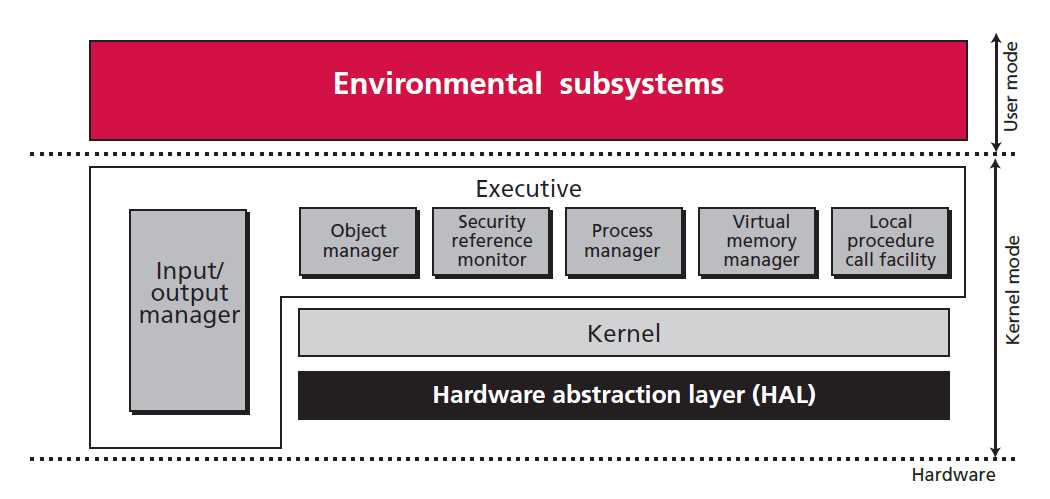
\includegraphics[width=0.85\textwidth]{\main/images/unit07/windows_architecture.png}
					\end{center}
					\begin{description}
						\item[Hardware Abstraction Layer (HAL)] Hides hardware differences from the upper layers.
						\item[Kernel] Heart of the operating system. Object-oriented software that sees any entity as an object.
						\item[Executive] Provides services for the whole OS. Runs in kernel (priveleged) mode. Made up of six subsystems: object manager, security reference monitor, process manager, virtual memory manager, local procedure call facility, and I/O manager.
						\item[Environmental Subsystems] Subsystems that allow Windows to run application programs designed for Windows, other operating systems, or earlier versions of Windows. The native subsystem that runs applications designed for Windows is \concept{Win32}. The environment subsystems run in the user mode.
					\end{description}
				\end{definition}
		\rulechapterend
\end{document}